% based on Model B of Software Development Life Cycles by Clif Kussmaul

\model{The Waterfall Model}

The following diagram shows the typical percentage of \textbf{total cost \& effort} for each stage of software development.
In practice, these percentages vary widely by project.

\begin{center}
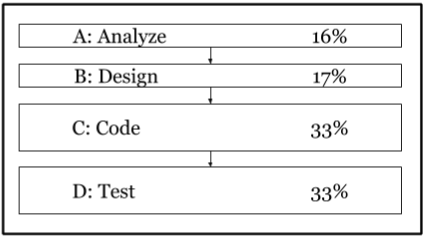
\includegraphics[scale=0.75]{waterfall.png}
\end{center}

\setlength{\defaultwidth}{10em}


\quest{10 min}


\Q Based on the Waterfall Model:

\begin{enumerate}%[itemsep=1ex]

\item How many stages are there?
\ans{4}

\item Which stage is 1st?
\ans{A:~Analyze}

\item Which stage(s) must be finished before \textbf{coding} starts?
\ans[12em]{A:~Analyze, B:~Design}

\end{enumerate}


\Q Based on the Waterfall Model:

\begin{enumerate}%[itemsep=1ex]

\item What \% of total effort is in the \textbf{last stage}?
\ans{33\%}

\item What \% of total effort is in the \textbf{first two stages}?
\ans{33\%}

\item When the project is \underline{25\%} completed, what \% of \textbf{analysis} is done?
\ans{100\%}

\item When the project is \underline{25\%} completed, what \% of \textbf{coding} is done?
\ans{0\%}

\item When the project is \underline{50\%} completed, what \% of \textbf{coding} is done?
\ans{About 50\%}

\item When the project is \underline{50\%} completed, what \% of \textbf{testing} is done?
\ans{0\%}

\end{enumerate}


\newpage

\Q It is important to find and fix errors in software.

\begin{enumerate}%[itemsep=1ex]

\item If \textbf{coding} errors are found during \textbf{C:~Code}, \\ in which stage should they be fixed?
\ans{C:~Code}

\item If \textbf{coding} errors are found during \textbf{D:~Test}, \\ in which stage should they be fixed?
\ans{D:~Test}

\item If \textbf{analysis} errors are found during \textbf{B:~Design}, \\ in which stage should they be fixed?
\ans{B:~Design}

\item If \textbf{analysis} errors are found during \textbf{D:~Test}, \\ in which stage should they be fixed?
\ans{D:~Test}

\item Which stage focuses most on \textbf{finding} errors?
\ans{D:~Test}

\item Are major errors in analysis and design more likely \\ when the project is \textbf{similar} to past projects, or \textbf{different}?
\ans{different}

\end{enumerate}


\Q Later stages often take more time, effort, and money than expected.
Explain why based on your answers to the previous questions.

\begin{answer}
Later stages must fix errors from earlier stages, and many errors are found late in the project during the Test stage.
\end{answer}
